\chapter{Motion of Rigid Bodies}
\label{chap:rbm}

In this chapter, we shall lay the foundations for analyzing the kinematics of a rigid or soft body in general space. Our goal is to present a geometric view of the translational and rotational rigid body motions. We take the classical screw theory approach owing to its simplicity in analyzing the geometry of kinematic motions compared against the common Denavit-Hartenberg (DH) conventions. We leave the treatment of the DH convention as an exercise for the reader. While the materials presented here may appear abstract, the applications are practical and useful. Therefore in reading the materials presented forthwith, it is recommended to the reader to ask what is it to the kinematic geometry of mechanisms that we have labored upon in \autoref{chap:intro}. The recommended texts for this chapter are 

\begin{itemize}
	\item Murray, R. M., Li, Z., \& Sastry, S. S. (1994). A Mathematical Introduction to
Robotic Manipulation . Book (Vol. 29), Chapter 2
	%
	\item A treatise on the theory of screws, Sir R.S. Ball, Chapter 1
	%
	\item Screw theory for robotics, Jose M. Pardos-Gotors, IROS2018 tutorial; (Email the instructor for a copy).
	%
\end{itemize}


\section{Screws}

Simply put, \textit{a screw is a line (called an axis) by which a definite linear magnitude (termed the pitch, $p$) is associated}.
%What follows is based on the thesis of Kenneth Salisbury~\cite{Salisbury}. 
%A \textit{screw} is defined collectively by a straight line in space called an \textit{axis} which has an associated \textit{pitch}, $p$, and a magnitude, $\ell$.  
A screw may be defined by a 6-vector of \textit{screw coordinates}, $\underline{s}=(S_1, S_2, S_3,S_4, S_5, S_6)$ which has the following interpretations in terms of the Pl\"ucker line coordinates of the axis
%
\begin{subequations}
	\begin{align}
	L &= S_1, \quad M = S_2, \quad N=S_3,   \label{eq:plucker_line} \\ 
	%
	P &= S_4 - pS_1, \quad Q = S_4 - pS_2, \quad R = S_6 - pS_3
	\label{eq:plucker_mom}
	\end{align}
\end{subequations}
%
where $L, M, N$ are proportional to the direction cosines of the line forming the axis while $P, Q, R$ are proportional to the moment of the line about the origin of the reference frame. If we scale the Plucker coordinates by $(L^2 + M^2 + N^2)^{1/2}$, the first three would represent the direction cosines of the line while the last three would represent the moments. We have the moment of the line as the cross product of a vector from the reference frame's origin to any point on the line with the unit vector in the line direction. Thus, we have the pitch of the screw defined as 
%
\begin{align}
	p = \dfrac{S_1\,S_4+S_2S_5+S_3S_6}{S_1^2+S_2^2+S_3^2}
\end{align}
%
whose magnitude is 
%
\begin{align}
	\|\ell \|^2 = S_1^2+S_2^2+S_3^2
\end{align}
%
for a finite pitch, otherwise, it is
%
\begin{align}
\|\ell \|^2 = S_4^2+S_5^2+S_6^2
\end{align}
%
for an infinite pitch. Note that  for infinitesimal screws, scalar multiplication and vector addition are valid so that two screws, $\underline{s}_1$ and $\underline{s}_2$ are considered linearly dependent if there exists non-zero scalars, $c_1$ and $c_2$ \ie $c_1\underline{s}_1+c_2\underline{s}_2=0$.


\subsection{Motion screws: Pitch, axis, twist}
%
The unique line about which a body in space rotates or translates for an infinitesimal motion or velocity of the body is called the \textit{twist axis}. Formally, we say \textit{a body receives a twist about a screw when it is uniformly rotated about the screw, while it is translated uniformly parallel to the screw, through a distance equal to the product of the pitch and the circular measure of the angle of rotation}~\cite{Ball}. Similar to the screw, the \textit{twist} is characterized by a six-vector of coordinates, $\underline{t}=(T_1, T_2, T_3, T_4, T_5, T_6)$ so that the components of the angular velocity of the body are denoted by $\underline{w}=(T_1, T_2, T_3)$ while the components of the linear velocity of a fixed point in the body lying at the origin of the coordinate system is $\underline{v}\equiv(T_4, T_5, T_6)$. Hence, we have the Pl\"ucker coordinates of the \textit{twist axis} given as
%
\begin{subequations}
	\begin{align}
	L &= T_1,\quad M=T_2, \quad N=T_3 \\
	%
	P &= T_4 - pT_1, \quad Q=T_5-pT_2, \quad R = T_6 - pT_3
	\end{align}
\end{subequations}
%
whereupon the pitch of the twist is 
%
\begin{align}
	p = \dfrac{T_1T_4+T_2T_5+T_3T_6}{T_1^2+T_2^2+T_3^2} = \dfrac{\underline{w}\cdot \underline
	{v}}{\underline{w}\cdot \underline{w} }.
	\label{eq:twist_pitch}
\end{align}


In screw theory, it is typical to concern ourselves only with the small displacements of a system's motion. Whenever a body admits an indefinitely small movement of a continuous nature, it is capable of executing that kind of movement denoted by a twist about a screw. When the body receives twists in several succession, the position that is finally attained is called the \textit{resultant twist}.

\noindent 
\begin{homework}
	What is the geometric meaning of \eqref{eq:twist_pitch} on a twist axis to you. Define \textit{pure rotation} and a \textit{pure translation} in terms of \eqref{eq:twist_pitch}\footnote{Figure out how they correspond to zero pitch and infinite pitch twists.}. 
\end{homework} 

\subsection{Dynamics screws: pitch, axis, twists}
%
For a set of forces and moments applied to a rigid body, there is a \textit{wrench axis}, a unique line, which has associated with it a pitch, $p$, and a magnitude. We may consider the set of forces and moments that act on the body to be a single force along  the wrench axis and a a moment about exerted about the axis. This force-moment pair is termed a \textit{wrench}, and it is characterized by the 6-vector $\underline{w} = (W_1, W_2, W_3, W_4, W_5, W_6)$. We consider the first three components of $\underline{w}$ to be the net force components, $\underline{f}$, exerted on the body and $\underline{m}=\{W_4, W_5, W_6\}$ to be the components of the net moment resolved at the origin of the reference frame. We define the Pl\"ucker coordinates of the \textit{wrench axis} as 
%
\begin{subequations}
	\begin{align}
	L &= W_1, \quad M=W_2, \quad N = W_3 \\
	P&= W_4-pW_1, \quad Q = W_5 - pW_2, \quad R=W_6 - pW_3
	\end{align}
\end{subequations}
%
with pitch defined as
%
\begin{align}
	p = \dfrac{W_1 W_4 + W_2 W_5 + W_3 W_6}{W_1^2 + W_2^2+W_3^2} = \dfrac{\underline{f} \cdot \underline{m}}{\underline{f} \cdot \underline{f}}.
	\label{eq:wrench_pitch}
\end{align}
%
Equation \eqref{eq:wrench_pitch} signifies that the pitch of the wrench is the ratio of the magnitude of the applied moment about a point to the magnitude of the applied force along a wrench axis. A \textit{zero pitch wrench}  would therefore correspond to pure force while an infinite pitch wrench would be a pure moment. We define the magnitude of the wrench as $\|\underline{f}\| = \sqrt{W_1^2 + W_2^2 + W_3^2}$ when we have a finite pitch. If the pitch in infinite, the magnitude is $\|\underline{m}\| = \sqrt{W_4^2 + W_5^2 + W_6^2}$.

\noindent 
\begin{homework}
	A unit screw, twist or wrench is one where the magnitude of the screw, twist or wrench is $1$.  
	
	(1). What is the geometric meaning of a unit screw to you? %Often with twist and wrenches we wish to associate a magnitude other than 1 so that there are $\infty^6$ different twists and wrenches if we consider their magnitudes as well. With this interpretation we can think of a unit screw as defining only an axis and a pitch. Then we can think of a given magnitude as defining a twist (if its units are rotation/time) or a wrench (if its units are force) acting along the screw. In both cases the pitch is expressed in length units. These six-spaces of (infinitesial) twists or wrenches can be considered to be vector spaces in tha t they are closed under vector addition and scalar multiplication.
	(2) Consult the identified reference materials and explain what a reciprocal screw is in no more than five sentences.
\end{homework}


\subsection{Screw Motions}

A \textit{screw motion} is a rotation about the axis, $l$ by an amount $\alpha = \ell$ followed by a translation by an amount $h\alpha$ that is parallel to the axis $l$. A pure translation occurs when $h=\infty$ so that the screw motion is composed of a \textit{pure translation} along the axis of the screw by a distance $\ell$. 



\section{Rodrigues' Formula}
%
The matrix exponential
%
\begin{align}
	e^{\hat{\omega}t} = I + \hat{\omega}t + \dfrac{(\hat{\omega}t)^2}{2!} + \dfrac{(\hat{\omega}t)^3}{3!} + \cdots
\end{align}
%
is instrumental in defining the rotation about an axis, $\omega$: 
%
\begin{align}
	R(\omega, \theta) = e^{\hat{\omega} \theta}.
\end{align}
%
Thus, for a matrix $\hat{\omega}$ in the Lie algebra ${so}(3)$, a unit vector $\|\omega\| = 1$, and a real number $\theta \in \bb{R}$, we write the exponential of $\hat{\omega} \theta$ as
%
\begin{align}
e^{\hat{\omega}\theta} = I + \theta \hat{\omega} + \dfrac{\theta^2}{2!}\hat{\omega}^2 + \dfrac{\theta^3}{3!}\hat{\omega}^3 + \cdots
\end{align}

\noindent 
\begin{homework}
	Given a matrix $\hat{m} \in so(3)$, suppose that the following relation holds,
	%
	\begin{align}
	\hat{m}^2 = m m^T - \|m\|^2 \identity \\
	%
	\hat{m}^3 = - \|m\|^2 \hat{m}
	\end{align}
	%
	with the fact that higher powers of $\hat{m}$ can be recursively found. Therefore, utilizing this lemma with $m =\omega \theta$, $\|\omega\| = 1$, show that 
	%
	\begin{align}
	e^{\hat{\omega}\theta}  = \identity + \hat{\omega} \sin \theta + \hat{\omega}^2(1 - \cos \theta).
	\label{eq:rodrigues}
	\end{align}
\end{homework} 
%
Equation \eqref{eq:rodrigues} is \textit{Rodrigues' formula}.


\section{The Matrix Exponential, The Lie Group and Lie Algebra}
%
For any matrix 
%
\begin{align}
\homo = \begin{bmatrix}
\rot & \disp \\
0 & 1
\end{bmatrix} \in SE(3) \text{ such that } \rot \in SO(3), \disp \in \bb{R}^3, \text{ and } \rot\rot^T = \identity
\end{align}
%
there exists a matrix 
%
\begin{align}
N = \begin{bmatrix}
\skew & x \\
0 & o
\end{bmatrix} \text{ such that } \skew = -\skew^T
\end{align}
%
such that $\exp(N) = \homo$ since we can write
%
\begin{align}
\begin{bmatrix}
\rot & \disp \\
0 & 1
\end{bmatrix}  
%
&=  \begin{bmatrix}
\identity & \disp \\
0 & 1
\end{bmatrix}
%
\begin{bmatrix}
\rot & 0 \\
0 & 1
\end{bmatrix}  =  \begin{bmatrix}
\identity & \disp \\
0 & 1
\end{bmatrix} 
%
\exp 
\begin{bmatrix}
\skew & 0 \\
0 & 0
\end{bmatrix}.
\label{eq:eulers_theorem}
\end{align}
%
We see that the exponential map is surjective onto $\bb{E}(3)$. $SE(3)$ is Lie Group whose isomorphism is the \textit{lie algebra} $\mathfrak{se(3)}$. 
Generally, \textit{we define the Lie Group \textit{SE(n)} on the configuration of a rigid body that consists of the pair $(p_{ij},\rot_{ij})$ to be the product space of $\bb{R}^n$ with \textit{SO(n}, called the \textbf{special Euclidean group}} \ie
%
\begin{align}
SE(n) = \{(p, R): p \in \bb{R}^n, \rot \in SO(n)\} = \bb{R}^n \times SO(n)
\label{eq:special_euclid3}
\end{align}

%
An element of $\mathfrak{se(3)}$\footnote{We typically write the Lie algebra in lowercase with the math frak style.} is the \textit{twist} earlier introduced, which is the infinitesimal generator of the Euclidean group. Formally, we define $\xi = (\omega, v) \in \bb{R}^6$ as the twist coordinates of $\hat{\xi}$. Equation \eqref{eq:eulers_theorem} is basically a re-statement of \textit{Euler's theorem, that is that a rigid body transformation is basically a rotation about a line passing through a preassigned fixed point}. 
Note that $\skew$ is the anti-symmetric matrix or skew-symmetric matrix with the following special property
%
\begin{align}
\skew(\overrightarrow{\omega}) = \hat{\omega} = \left(\begin{array}{ccc}
0 & -\omega_z & \omega_y \\
%
\omega_z & 0 & -\omega_x \\
%
-\omega_y & \omega_x & 0
\end{array}\right)
\end{align}
%
that is $\omega_x, \omega_y, \omega_z$ are the component of the vector $\overrightarrow{\omega}$ such that 
\[
s_{ij} = \begin{cases}
0, \quad \text{if } i = j \\
-s_{ji} \quad \text{ if } i \neq j.
\end{cases}
\]
%
It is a common convention in robotics texts to denote the skew symmetric matrix by $\hat{\omega}$ and we will adopt that convention for the rest of these notes. 
%
\begin{figure}[tb!]
	\centering
	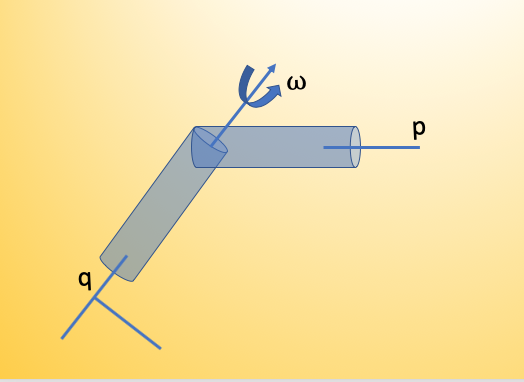
\includegraphics[width=.6\columnwidth]{figures/revolute.png}
	\caption{Illustration of rotation of interconnecting link of two spherical links.}
	\label{fig:revolute_point}
\end{figure}
%
In particular, we define the \textit{homogeneous coordinates} for a point $q \in \bb{R}^3$ that is rotating about an axis $\overrightarrow{\omega} \in \bb{R}^3$ such that $\|\overrightarrow{\omega}\| = 1$ (see \autoref{fig:revolute_point}) as 
%
\begin{align}
\hat{\xi} = \homo^{-1} \dot{\homo} = \left(\begin{array}{cc}
\hat{\omega} & v \\
%
0 & 0
\end{array}\right) \in \mathfrak{se}(3)
\label{eq:twist_defo}
\end{align}
%
where $v = -\omega \times q$. Equation \eqref{eq:twist_defo} is the object's velocity in the body frame; essentially the \textit{Lie algebra element} and we can obtain the twist coordinates from it via the so-called \textit{wedge operator} 
%
\begin{align}
\left(\begin{array}{c}
\hat{\omega} 
\\ 
v 
\end{array}\right)^{\wedge} = \left(\begin{array}{cc}
\hat{\omega} & v \\
%
0 & 0
\end{array}\right).
\end{align}
%
If the link of \autoref{fig:revolute_point} moves at a unit velocity, we can write the velocity at the tip point as 
%
\begin{align}
\dot{p} = \omega \times (p(t) - q(t)) 
\end{align}
%
where $p(t), q(t)$ are the paths traced out by points $p$ and $q$ respectively during the motion.
%

We define the exponential for  the matrix $A\in SO(n)$, which is a component of the solution to the ordinary differential equation, $\dot{x}(t) = A x(t)$ where $x(t) \in \bb{R}^n$ as 
%
\begin{tcolorbox}[title=The Matrix Exponential]
\begin{align}
e^{At} = \identity +  At + \dfrac{A^2t^2}{2!} + \dfrac{A^3 t^3}{3!} + \ldots 
\label{eq:matrix_exponential}
\end{align} 
\end{tcolorbox}
%

For the matrix exponential  of \eqref{eq:matrix_exponential}, we would like to write the equation in a closed-form expression since we are interested in definite solutions for our forward kinematics problems. For suppose that some matrix $D \in \bb{R}^{n\times n}$ and $P\in \bb{R}^{n\times n}$ are available, then we find that 
%
\begin{align}
e^{At} &= \identity + (PDP^{-1})t  + (PDP^{-1})(PDP^{-1})\dfrac{t^2}{2!}  + \ldots \nonumber \\
& = P\left(\identity  Dt + \dfrac{(Dt)^2}{2!} + \ldots \right)P^{-1} \\
& = P e^{Dt}P^{-1}.
\end{align}
%
\begin{definition}[Exponential Map Properties]
	%
	We note the following properties of the matrix exponential:
	
	\begin{inparaenum}
		\noindent(1) $d(e^{At}) = Ae^{At} = e^{At} A$.\\
		%
		(2) For $A=PDP^{-1}$ for some diagonal $D\in \bb{R}^{n\times n}$ and an invertible $P\in \bb{R}^{n\times n}, \,e^{At}=P e^{Dt}P^{-1}$.\\
		%
		(3) For $AB = BA$, we have $e^Ae^B = e^{A+B}$. \\
		%
		(4) $(e^A)^{-1} = e^{-A}$
		%
	\end{inparaenum}
	\label{def:exp_map}
\end{definition}
%

For the mapping from the twist map in the Lie algebra to the Lie group notation, we have the following:
%
\begin{tcolorbox}[title=Exponential map from $\mathfrak{se}(3)$ to $SE(3)$]
	\begin{align}
	e^{\hat{\xi \theta}} = \left(\begin{array}{cc}
	e^{\hat{\omega \theta}} & (\identity - e^{\hat{\omega} \theta}) (w \times v) + \omega \omega^T v \theta\\
	%
	0 & \identity
	\end{array}\right) \in SE(3)
	\end{align}
\end{tcolorbox}
%



\subsection{The Lie Group Notations}
\begin{figure}[tbph]
	\centering
	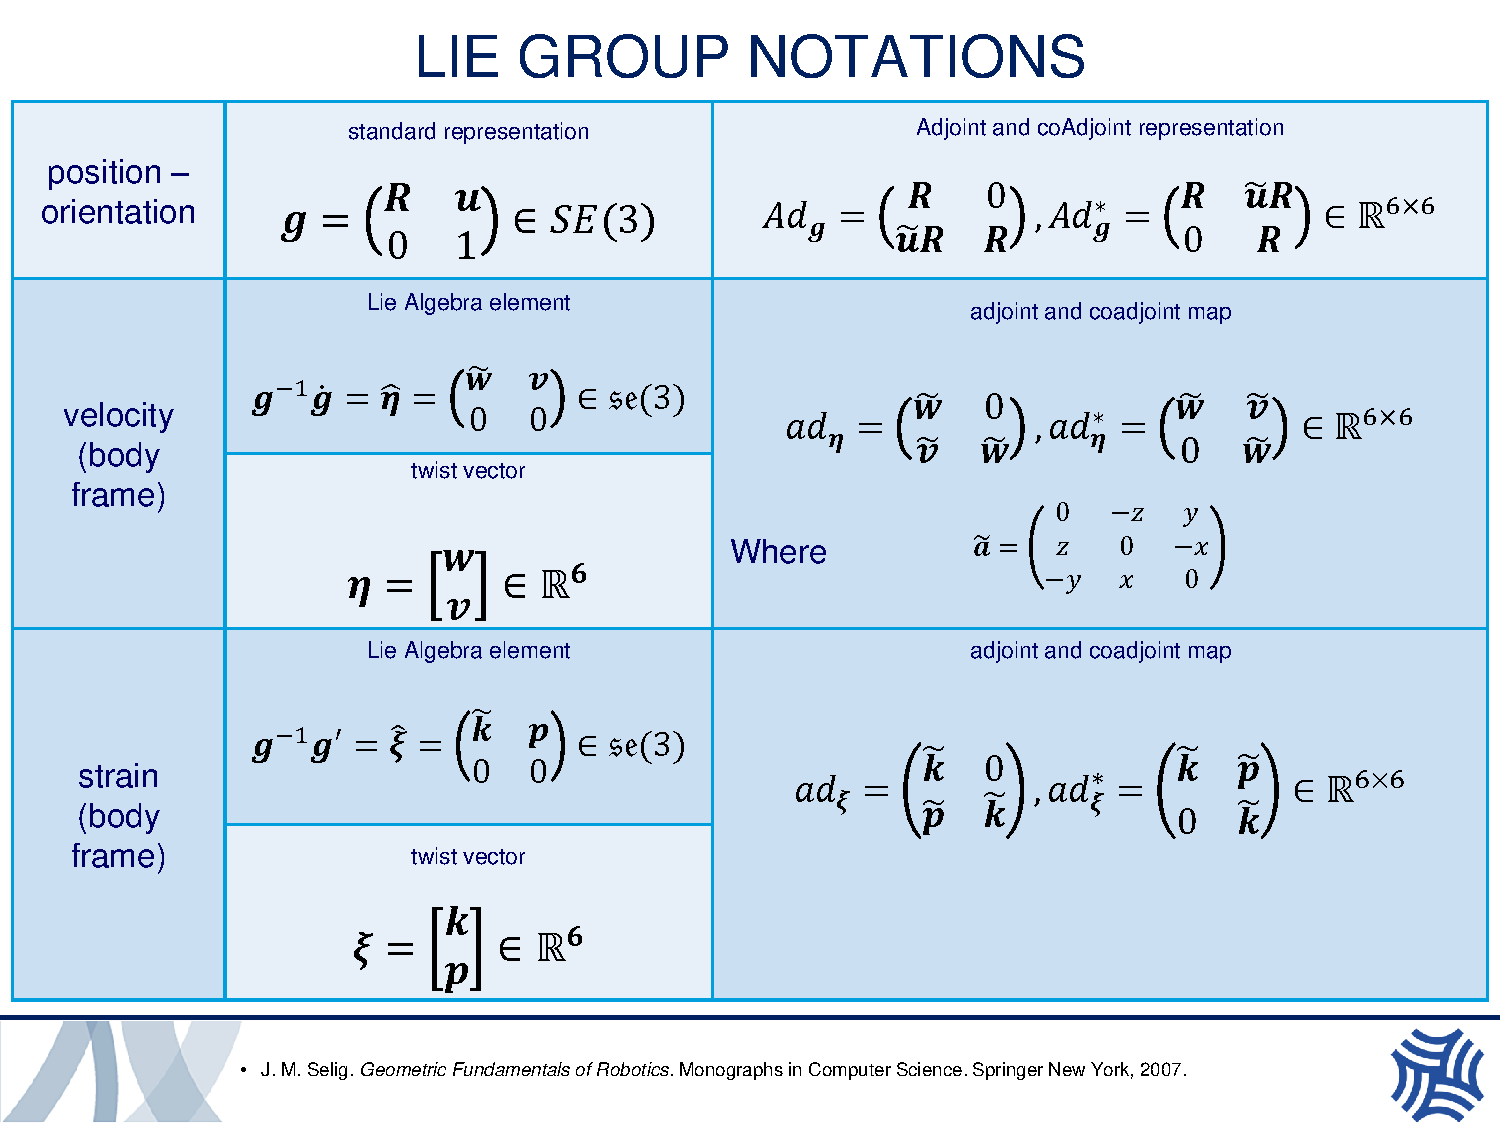
\includegraphics[width=\columnwidth]{figures/lienotations.pdf}
	\caption{Lie Group and their Notations. Reprinted with permission from Federico Renda. IROS 2018, Screw Theory Tutorial.}
	\label{fig:lienotations}
\end{figure}

\subsection{Exponential Map and Kinematic Chains}
\label{subsec:matexp}

Now consider a robot manipulator of the form shown in \autoref{fig:staubli}. The reader may imagine that there are right-handed triads of orthogonal vectors at the tip of each link of the chain so that the Euclidean transformation that describes the position and orientation of the $(i+1)'th$ link with the $i'th$ link is 
%
\begin{align}
\left(\begin{array}{cc}
\rot_i & \disp_i \\
0 & 1
\end{array}\right) \text{ exp } \left(\begin{array}{cc}
\skew_i & 0 \\
0 & 0
\end{array}\right)  \theta_i =  \homo_i \text{ exp } (\hat{\omega_i} \theta_i)
\end{align}
%
and we may imagine the triad that is fixed at the end-effector to be related to the triad at the base of the robot by the following relation
%
\begin{align}
H(\theta_1, \theta_2, \cdots, \theta_n) = \rot_1\,e^{\theta_1 \hat{\omega}_1}\,
%
\rot_2\,e^{\theta_2 \hat{\omega}_2},\, \cdots, 
%
\rot_n\,e^{\theta_n \hat{\omega}_n}\,	
\end{align}
%
and since $P exp(M) P^{-1} = exp(PMP^{-1})$, we can write the \textit{forward kinematic map}, $g_{st}: Q \rightarrow SE(3)$ as 
%
\begin{figure}[t!]
	\centering
	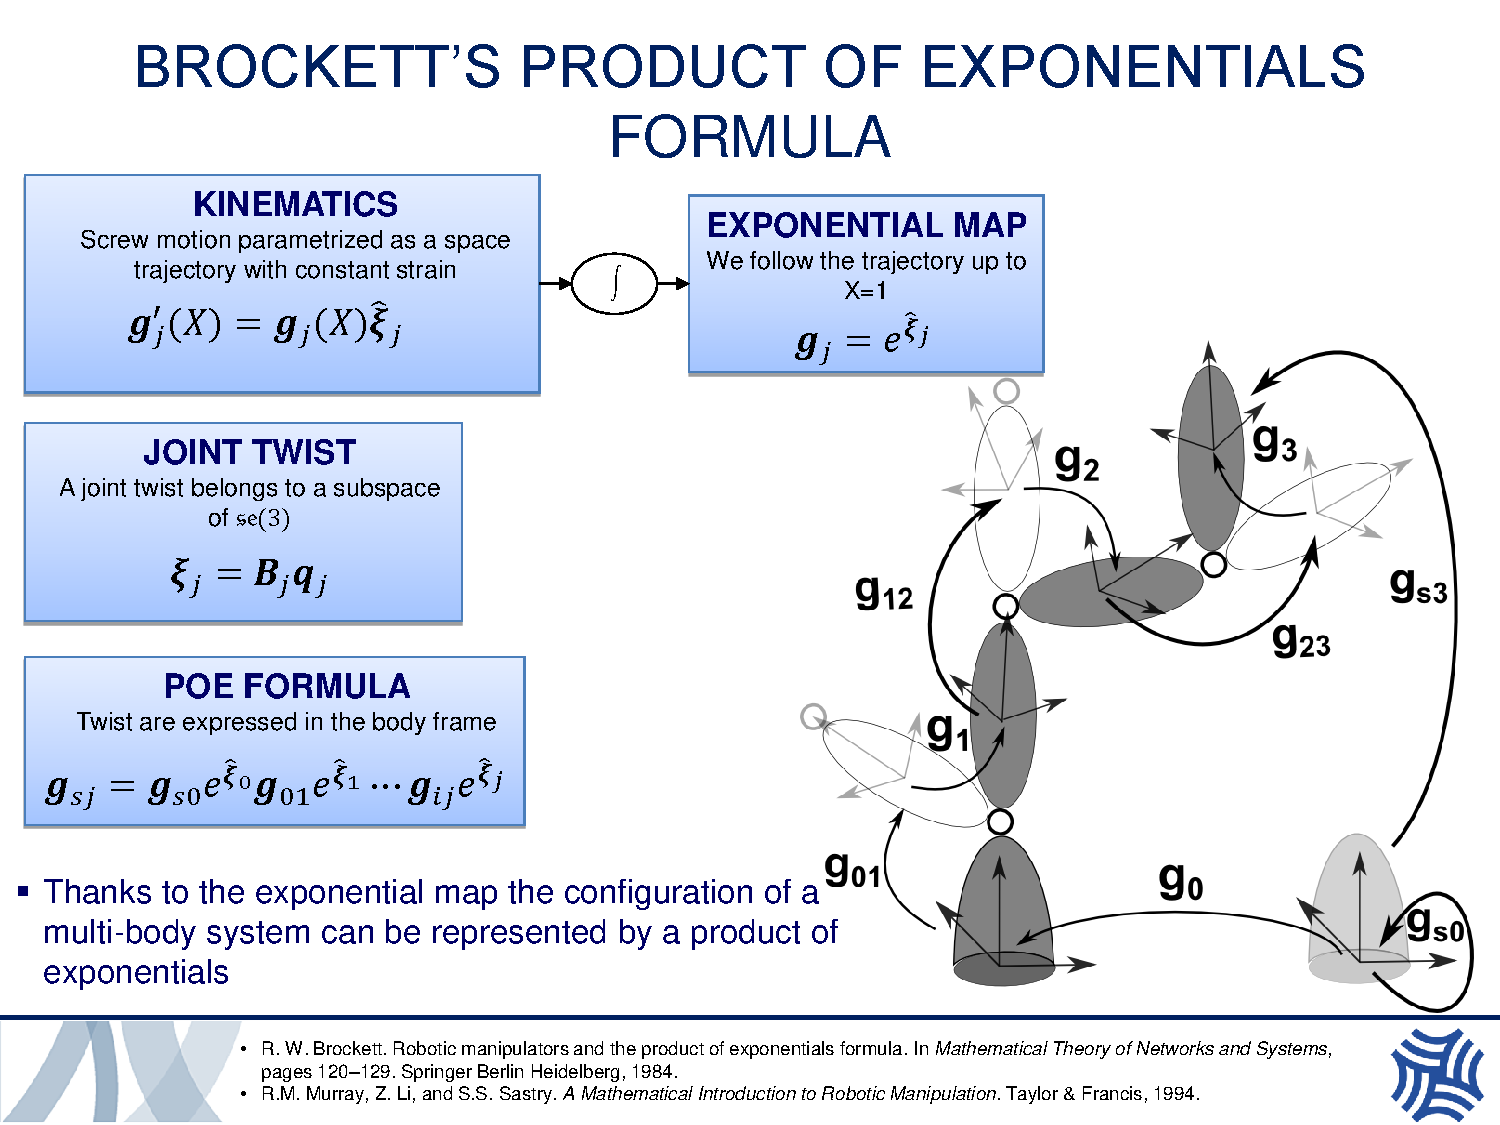
\includegraphics[width=\columnwidth]{figures/brockettpoe.pdf}
	\caption{An illustration of the exponential map for a multi-body rigid system. Reprinted with permission from Federico Renda. IROS 2018, Screw Theory Tutorial.}
	\label{fig:brockettpoe}
\end{figure}
%
\begin{align}
g_{st}(\theta) = e^{\theta_1 \hat{\omega}_1}\,
%
\,e^{\theta_2 \hat{\omega}_2}\, \cdots, 
%
\,e^{\theta_n \hat{\omega}_n}\,g_{st}(0)
\end{align}
%
using the identity repeatedly.
%
\section{Rigid Body Transformations}

A rigid body motion is one that preserves the  distance between points. In classical mechanics, we are concerned about the material description of a rigid body whereby we consider all the particles that make up the rigid body as a whole rather than treat them as a continuum as it is typical in continuum mechanics.  Therefore by this logic, \textit{a rigid body is a collection of particles by which the distance between any two particles remain fixed, irrespective of the motions of the body or forces exerted on that body~\cite{MurrayBook}}. 

Suppose we have two points $a$ and $b$ on a rigid body, we must have
%
\begin{align}
\|a(t_f) - b(t_f)\| = \|a(t_i) - b(t_i)\|
\end{align}
%
where $t_i$ and $t_f$ are two instants of time that the two points \ie $a$ and $b$ are observed on the rigid body. We thus see that distance is preserved irrespective of observer placement in rigid body transformations. For continuum-based systems such as soft robots, this is not so and we often need to come up with clever mechanisms of characterizing the motion of its particles. 

\noindent \textbf{Definition}: A mapping $g: \bb{R}^3\rightarrow\bb{R}^3$ is a \textit{rigid body transformation} if it satisfies the following properties:
\begin{itemize}
	\item Length is preserved \ie $\|g(a) - g(b)\| = \|a-b\|$ for all point $a, b \in \bb{R}^3$.
	%
	\item The cross product for all vectors is preserved \ie $g(p \times q) = g(p) \times g(q)$ where $p, q \in \bb{R}^3$ .
\end{itemize}
%
This means that the inner product is preserved so that we have, 
\begin{align}
p^Tq = g(p)^T \times g(q).
\end{align}
%
It follows that orthogonal vectors are transformed to orthogonal vectors and since cross product is naturally preserved, rigid body transformations map orthonormal coordinate frames to orthonormal coordinate frames. Note that it is possible to have rotation of particles despite the two strong forms presented above. To track the location of a rigid body in space, it therefore follows that we need to keep track of the motion of any one point as well as the rotation of the rigid body about this point. Therefore, the \textit{configuration} of the rigid body is found by attaching a Cartesian coordinate frame to a point on the rigid body and keeping track of the motion of the body coordinate frame with respect to a fixed frame. To ease representation, we typically require that all coordinate frames be \textit{right-handed}: given three Cartesian orthonormal vectors $\bm{x}, \bm{y}, \bm{z} \in \bb{R}^3$ which characterize the motion of a coordinate frame, they must satisfy $\bm{z} = \bm{x} \times \bm{y}$.


Going by the definitions of twist in the foregoing, it follows that a twist is to a rigid body what a vector is to a point. They both express the relation needed to transfer an object from one given position to another. When a body twists at an instant, the screw about which it twists is referred to as the \textit{instantaneous screw}.

\subsection{Translation in $\bb{R}^3$}

%
For the two coordinate frames shown in  \autoref{fig:2_coords}, say we choose the $o_0x_0 y_0$ frame as the reference and the $o_1x_1y_1$ as the moving coordinate frame, the way we would characterize the translation motion of the the point $q$ would be to represent its translation from the reference frame by the Cartesian displacement along $x$ and $y$ so that we have 
\begin{figure}
	\centering
	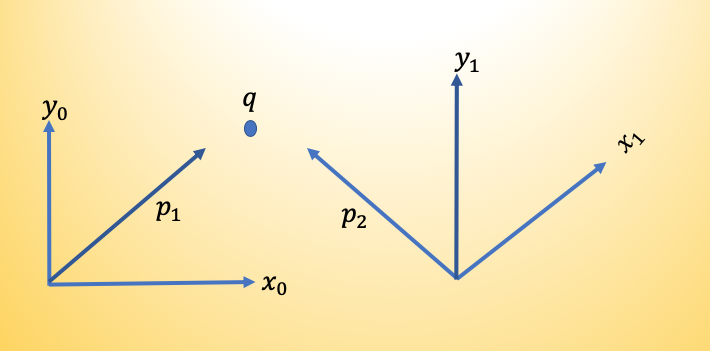
\includegraphics[width=.8\columnwidth]{figures/trans_coords.png}
	\caption{A point $q$ in space with respect to two coordinate frames.}
	\label{fig:2_coords}
\end{figure}
%
\begin{align}
q^0 = \left( \begin{array}{c}
q^0_x \\ q_y^0
\end{array}
\right), \quad
%
q^1 = \left( \begin{array}{c}
q^1_x \\ q_y^1
\end{array}
\right)
\end{align}
%
where the superscript denotes the reference frame and the subscript denotes the coordinate of the point $q$ along an axis in either Cartesian frame. The origin of the two frames are both points in space; therefore, the we can assign the coordinates that denote the position of the origin of one coordinate frame with respect to another as 
%
\begin{align}
o^0_1 = \left( \begin{array}{c}
o^0_x \\ o^0_y
\end{array}
\right), \quad
%
o^1_0 = \left( \begin{array}{c}
o^1_x \\ o^1_y
\end{array}
\right).
\end{align}
%
For vectors such as twists or wrenches, we use a similar notation as those used for points. Thus if $p_1, p_2$ are two vectors that are invariant with respect to the choice of coordinate frames, we would have
%
\begin{align}
p^0_1 = \left( \begin{array}{c}
o^0_x \\  o^0_y
\end{array}
\right)^T,
%
\quad p^1_1 = R(-\theta) q^0, 
%
\quad p^0_2 = R(\theta) q^0, \quad p^1_2 = \left( \begin{array}{c}
o^1_x \\  o^1_y
\end{array}
\right)^T
\end{align}
%
where $\theta$ is the angle that coordinate frame $1$ makes with respect to coordinate frame $0$. In robotics, the standard way to apply a rotation is counterclockwise. This is the reason we negate the angle of rotation when finding the vector $p_1$ in frame $1$. We will introduce the definition of the rotation matrix $R$ shortly. Performing frame transformations is a fundamental step to getting a robot work as envisioned. We must ensure that all coordinate vectors are defined with respect to the same coordinate frame. We say two vectors are ``equal" when they have the same magnitude and direction. Therefore, for vectors that are not constrained to be located at the same point in space, we require that they defined with respect to frames whose coordinates are parallel, given that absolute locations are not consequential, but the magnitude and direction of the vector.

\subsection{Rotations in $\bb{R}^3$}
%
We would like to establish a convention  that all coordinate frames will be right-handed. Our goal is to establish the orientation of an object by specifying the local coordinate on the body; we then describe the body's \textit{relative orientation} between a coordinate frame attached to the body and a fixed or an inertial coordinate frame. 
%
\begin{figure}[tb!]
	\centering
	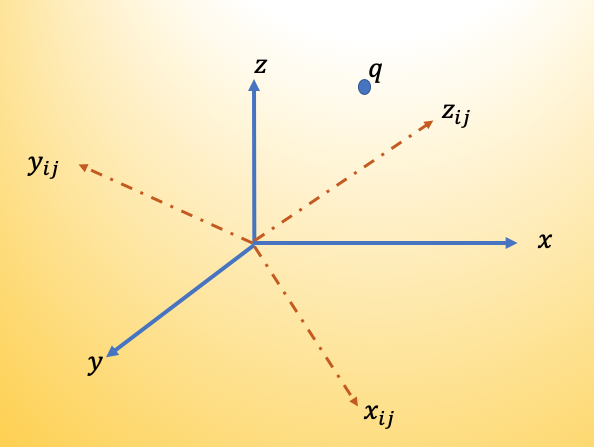
\includegraphics[width=\columnwidth]{figures/rotation_illus.png}
	\caption{An illustration of the relative orientation of a rigid object $q$ between an inertial frame $I$ and a body frame $J$.}
	\label{fig:rotation_illus}
\end{figure}
%
Suppose that we have two frames $I$ and $J$, where $I$ is the inertial frame, while $J$ is the body frame as shown in \autoref{fig:rotation_illus}. Let $\bm{x}_{ij}, \bm{y}_{ij},\bm{z}_{ij} \in \bb{R}^3$ be the coordinates of the principal axes of $J$ relative to $I$ so that we have the following matrix as a result of composing the respective coordinate vectors
%
\begin{align}
R_{ij} = \begin{bmatrix}
\bm{x}_{ij} \quad  \bm{y}_{ij} \quad \bm{z}_{ij}
\end{bmatrix} = \begin{bmatrix}
r_{11} &  r_{12} & r_{13} \\
r_{21} & r_{22} &  r_{23} \\
r_{31} & r_{32} &  r_{33}
\end{bmatrix}.
\label{eq:rotation_compoz}
\end{align}
%
The resulting matrix in \eqref{eq:rotation_compoz} is the \textit{rotation matrix}. This matrix can be rewritten by noting that the components of a vector are the projections of that vector onto the unit directions of its reference frame. Thus, the components if $R_{ij}$ in \eqref{eq:rotation_compoz} can be written as the dot product of a pair of unit vectors:
%
\begin{align}
R_{ij} = \begin{bmatrix}
\bm{x}_j \cdot \bm{x}_i & \bm{y}_j \cdot \bm{x}_i & \bm{z}_j \cdot \bm{x}_i \\
%
\bm{x}_j \cdot \bm{y}_i & \bm{y}_j \cdot \bm{y}_i & \bm{z}_j \cdot \bm{y}_i \\
%
\bm{x}_j \cdot \bm{z}_i & \bm{y}_j \cdot \bm{z}_i & \bm{z}_j \cdot \bm{z}_i 
\end{bmatrix}.
\label{eq:direction_cosines}
\end{align}
%
The components of the rotation matrix \eqref{eq:rotation_compoz} are sometimes called direction cosines since the dot product of two unit  vectors give the cosine of the angle between them as shown in \eqref{eq:direction_cosines}. If we examine the rows of \eqref{eq:direction_cosines}, we see that the rows of $R_{ij}$ are the unit vectors coordinates of $I$  in the frame $J$ so that we have 
%
\begin{align}
R_{ij} = R_{ji}^T
\end{align}
%
which is to say that the inverse of the rotation matrix is equal to its transpose. 
Noting that $\|\bm{r}\|^2 = x_i^2 + y_j^2+z_i^2 = 1$,  $r_i \cdot r_j = 0$ when $i \neq j$, and $r_i \cdot r_i = 0$, this can be thus verified as 
%
\begin{align}
R_{ij}^T \cdot R_{ji} & = 
\begin{bmatrix}
\bm{x}_j \cdot \bm{x}_i & \bm{x}_j \cdot \bm{y}_i  & \bm{x}_j \cdot \bm{z}_i \\
%
\bm{y}_j \cdot \bm{x}_i & \bm{y}_j \cdot \bm{y}_i & \bm{y}_j \cdot \bm{z}_i \\
%
\bm{z}_j \cdot \bm{x}_i & \bm{z}_j \cdot \bm{y}_i  & \bm{z}_j \cdot \bm{z}_i 
\end{bmatrix}
\cdot 
\begin{bmatrix}
\bm{x}_j \cdot \bm{x}_i & \bm{y}_j \cdot \bm{x}_i & \bm{z}_j \cdot \bm{x}_i \\
%
\bm{x}_j \cdot \bm{y}_i & \bm{y}_j \cdot \bm{y}_i & \bm{z}_j \cdot \bm{y}_i \\
%
\bm{x}_j \cdot \bm{z}_i & \bm{y}_j \cdot \bm{z}_i & \bm{z}_j \cdot \bm{z}_i 
\end{bmatrix} \\
%
& = 
\begin{bmatrix}
\bm{x}_j \cdot \bm{x}_j \cdot \|\bm{r}\|^2 & \bm{x}_j \cdot \bm{y}_j \cdot \|\bm{r}\|^2 & \bm{x}_j \cdot \bm{z}_j  \cdot \|\bm{r}\|^2  \\
%
\bm{y}_j \cdot \bm{x}_j  \cdot \|\bm{r}\|^2  & \bm{y}_j \cdot \bm{y}_j  \cdot \|\bm{r}\|^2  & \bm{y}_j \cdot \bm{z}_j  \cdot \|\bm{r}\|^2  \\
%
\bm{z}_j \cdot \bm{x}_j  \cdot \|\bm{r}\|^2  & \bm{z}_j \cdot \bm{y}_i  \cdot \|\bm{r}\|^2  & \bm{z}_j \cdot \bm{z}_j  \cdot \|\bm{r}\|^2  
\end{bmatrix}
%
= 
\left(\begin{array}{ccc}
1 & 0 & 0 \\
%
0 & 1 & 0  \\
%
0 & 0 & 1 
\end{array}\right) \\
%
& = \bm{I}_3
\end{align}
%
where $\bm{I}_3$ is the $3 \times 3$ identity matrix.
%

\noindent 
\begin{homework}
	Verify that $R_{ij} = R_{ji}^{-1} \equiv R_{ji}^T$. Furthermore, verify that the determinant of the rotation matrix is $\pm1$ \ie $det R = \pm1$.
\end{homework}

The determinant of the $R$ matrix is written as 
%
\begin{align}
\text{det }  R = r_1^T \left(r_2 \times r_3\right).
\end{align}
%
For right-handed coordinate frames, we have that $r_2 \times r_3 = r_1$ so that $r_1^Tr_1 = 1$ for a coordinate frame that aligns with the right-hand orthonormal frame representation. This special property that a $3 \times 3$ matrix satisfies $r_2 \times r_3 = r_1$ and that $\text{det }  R = r_1^Tr_1 = 1$ is called the special orthogonal property, denoted \textit{SO(3)}. Special orthogonal means $\text{det } R = + 1$. The set of all SO matrices in $\bb{R}^{n\times n}$ is defined by 
%
\begin{align}
SO(n) = \{R\in \bb{R}^{n\times n}: RR^T = \bm{I}, \text{det } R = + 1\}.
\end{align}

\subsection{Rotation Matrices as Transformations}
%
Suppose we are tasked with transforming a point $q$ from one coordinate frame  $J$ to a frame $I$ based on  \autoref{fig:rotation_illus}. Suppose that $q_j = (x_j, y_j, z_j)$ are the coordinates of $q$ with respect to the frame $J$. We may reason that $x_j, y_j, z_j \in \bb{R}^3$ are the projections of $q$ onto the coordinate axes of $B$, which in turn, have coordinates $\bm{x}_{ij}, \bm{y}_{ij},\bm{z}_{ij} \in \bb{R}^3$ with respect to coordinate frame $I$; then it follows that the coordinates of $q$ relative to frame $I$ is
%
\begin{align}
q_i = \bm{x}_{ij} x_j + \bm{y}_{ij} y_j + \bm{z}_{ij} z_j.
\end{align}
%
which in vectorized form is 
%
\begin{align}
q_i & = \left(\begin{array}{ccc}
\bm{x}_{ij} &  \bm{y}_{ij} & \bm{z}_{ij}
\end{array}\right)
%
\left(\begin{array}{c}
x_j \\ y_j \\ z_j
\end{array} \right) 
& = R_{ij}q_j
\end{align}
%
where the last part of the above equation follows from \eqref{eq:direction_cosines}.

Just as a rotation matrix can act on points to transform them in the world, so can rotation matrices act on vectors. Say we have another point $p_j$ on the frame $J$ in \autoref{fig:rotation_illus}, then the vector that connects a point $q_j$ in the frame $J$ to $p_j$ is $v_j = q_j - p_j$ so that the action of the rotation matrix on $v_j$ is
%
\begin{align}
R_{ij}(v_j) := R_{ij} q_j - R_{ij} p_j = q_i - p_i = v_i.
\end{align}


\subsection{Planar Rotations}
%
We now revisit the relative orientation between two coordinate frames as shown in \autoref{fig:rotation_illus}. Suppose now that the angle of rotation between the two coordinate frames is $\theta$ as shown in \autoref{fig:planar_rot}, it follows that 
%
\begin{figure}[tb!]
	\centering
	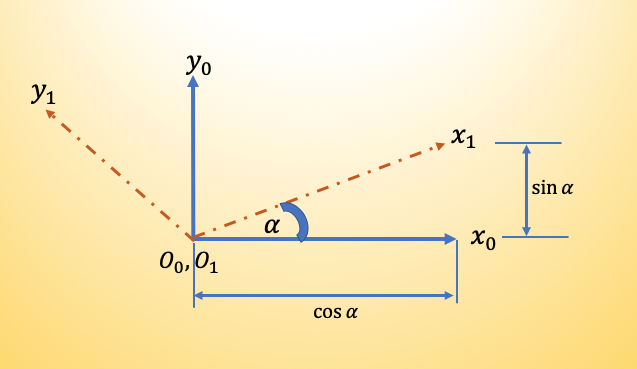
\includegraphics[width=.75\columnwidth]{figures/planar_rot.png}
	\caption{Illustration of rotation between two frames in a plane.}
	\label{fig:planar_rot}
\end{figure}
%
the composition of the rotation allows us to write 
%
\begin{align}
R_1^0 = \left(\begin{array}{cc}
x_1^0 \,\,| & y_1^0
\end{array}\right)
\end{align}
%
whereupon $x_1^0$ and $y_1^0$ have the usual meanings as before and are expressed as 
%
\begin{align}
x_1^0 = \left(\begin{array}{cc}
\cos \alpha \\ \sin \alpha
\end{array}\right) \text{ and }
%
y_1^0 = \left(\begin{array}{cc}
-\sin \alpha \\ \cos \alpha
\end{array}\right)
\end{align}
%
so that composing the rotation matrix, we have
%
\begin{align}
R = \left(\begin{array}{cc}
\cos \alpha & -\sin \alpha \\ \sin \alpha &  \cos \alpha
\end{array}\right)
\end{align}
%
While you might find the above approach rather daunting, an easier geometric way to visualize the transformation of matrices is to recall that the columns of the rotation matrix are the direction cosines of the coordinate axes of $o_1x_1y_1$ relative to the coordinates of $o_0x_0y_0$ \cf \eqref{eq:direction_cosines}. For a planar rotation, we could extract the first $2\times 2$ block of \eqref{eq:direction_cosines} so that 
%
\begin{align}
R_1^0 = \begin{bmatrix}
\bm{x}_0 \cdot \bm{x}_1 & \bm{y}_1 \cdot \bm{x}_0 \\
%
\bm{x}_0 \cdot \bm{y}_1 & \bm{y}_1 \cdot \bm{y}_0
\end{bmatrix} 
\end{align}
%
And since the dot product of two vectors is basically the cosine of the angles between them, we have
%
\begin{align}
R_1^0 =  \begin{bmatrix}
cos \alpha &  -cos(\pi/2 - \alpha) \\
%
cos(\pi/2 - \alpha) & cos \alpha
\end{bmatrix} 
%
=  \begin{bmatrix}
cos \alpha &   - \sin \alpha  \\
%
\sin \alpha  & cos \alpha
\end{bmatrix} 
\end{align}
%
Note the way the negative signs have entered the matrix due to the counterclockwise direction of rotation that we have chosen so as to preserve the positiveness of the determinant of $R$. In particular, the projection of $y_1$ on $x_0$ is negative because of our right-handed frame.

\noindent 
\begin{homework}
	Compose the rotation matrix in three dimensions where all axes of the inertial frame are rotated by an angle $\beta$ around each of the $x_0$, $y_0$ and $z_0$ axes respectively using the foregoing logic. In addition, for each transformation, verify that (1) $R_{e, \beta} = I$ where $e$ is the axes about which we are rotating and $\beta$ is the angle of rotation, (2) the composition of rotations about the angles $\beta$ and $\alpha$ in a successive manner implies that $R_{z, \beta}, R_{z, \alpha} = R_{z, \beta + \alpha}$, and (3) ${(R_{z, \beta})}^{-1} = R_{z, -\beta}$. Bonus points will be awarded for cool 3D visualizations.
\end{homework} 

\begin{figure}[tb!]
	\centering
	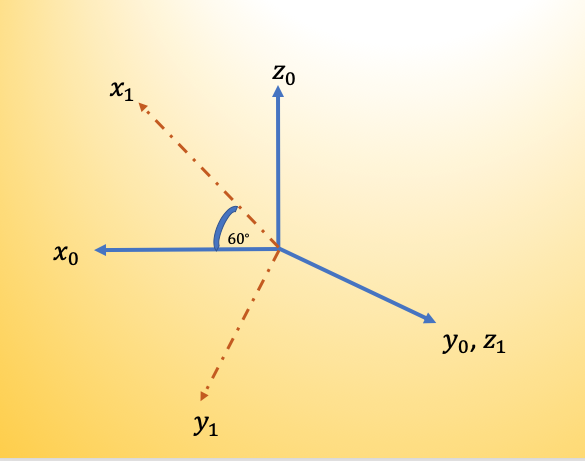
\includegraphics[width=.8\columnwidth]{figures/two_frames.png}
	\caption{Relative orientation between two frames.}
	\label{fig:two_frames}
\end{figure}


\noindent 
\begin{homework}
	For the two frames shown in \autoref{fig:two_frames}, determine the rotation matrix between them. In addition, explain the difference between rotating about a \textit{current frame} and rotating about a \textit{fixed frame}\footnote{See sections 2.4.1 and 2.4.2 of Spong's book.}. In particular, when is it necessary to carry out a \textit{pre-multiplication} and when is it necessary to carry out a \textit{post-multiplication} when transforming points or vectors about coordinate frames?
\end{homework}

\begin{tcolorbox}[title=Order of rotations]
	%
	A rotation about a fixed axis necessarily means a \textbf{pre-multiplication} while a rotation about a current axis necessitates a \textit{post-multiplication}.
\end{tcolorbox}


\subsection{Composition of Rotations}
%
Rotations matrices have this desirable property that they can be composed together to form transform a point between successive frames. Take for example a frame $K$ whose orientation relative to frame $J$ is $R_{jk}$, and frame $J$ whose orientation relative to frame $I$ is $R_{ij}$, we can write out the orientation of frame $K$ relative to $I$ as 
%
\begin{align}
R_{ik} = R_{ij} R_{jk}.
\label{eq:current_frame_rotation}
\end{align}
%
The rotation described above would be equivalent to rotating frame $K$ relative to frame $I$ according to $R_{ij}$, then aligning frame $J$  to $K$, we rotate $K$ relative to $I$ according to $R_{jk}$. The resulting frame $K$ has orientation with respect to $I$ given by $R_{ij} R_{jk}$. This frame relative to which rotation occurs is termed the \textit{current frame}.

\noindent 
\begin{homework}
	For the robot manipulator we are using in this class, suppose that you have the following point in the base frame of the robot, $q_o = [-2, 3, 1]$. Furthermore, suppose that the joint angles for all six joints are respectively $\{-90, 60, 30, 45, 90, 125 \}$, transform the point $q_0$ in the base frame to a coordinate frame on the sixth joint.
\end{homework}

%
\begin{tcolorbox}[title=Properties of Rigid Body Rotation Matrices]
	\textit{Rigid body} rotations preserve
	\begin{itemize}
		\item distance: $\|Rq - Rp\| = \|q-p\|$ for all $q, p \in R^3$
		%
		\item orientations: $R(i \times j) = Ri \times Rj$ for all $i, j \in \bb{R}^3$.
	\end{itemize}
\end{tcolorbox}

What follows is adapted from Figure 2.5 from Spong and Vidyasagar's book. It is meant to illustrate the rotation applied to a point from one frame to another.
%
\begin{figure}[tb!]
	\centering
	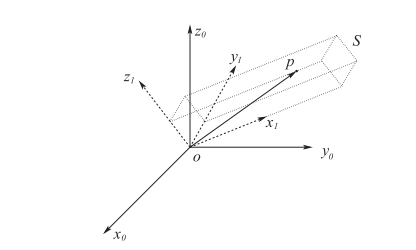
\includegraphics[width=.8\columnwidth]{figures/point_transform.png}
	\caption{Coordinate frames on a body. Reprinted from \cite{SpongBook}}.
	\label{fig:point_transform}
\end{figure}

For consider \autoref{fig:point_transform} whereupon the rigid body $S$ has a coordinate frame $o_1x_1y_1$ attached. For the coordinates of the point p with respect to frame $o_1x_1y_1$ or $p^1$, we are tasked with finding the coordinates of $p$ relative to a fixed reference frame $o_0x_0y_0$. We note that $p^1 = [u, v, w]^T$ satisfies 
%
\begin{align}
p = ux_1 + v y_1 + w z_1.
\label{eq:point_transform1}
\end{align}
%
Matter-of-factly, the coordinates of $p^0$ can be obtained based on the projection trick we introduced earlier by projecting $p$ onto the coordinate axes of $o_0x_0y_0z_0$ so that we have 
%
\begin{align}
p^0 = \left(\begin{array}{c}
p \cdot x_0 \\ p \cdot y_0 \\ p \cdot z_0
\end{array}\right)
\label{eq:point_transform2}
\end{align}
%
so that substituting \eqref{eq:point_transform1} into \eqref{eq:point_transform2}, we have
%
\begin{align}
p^0 = \left(\begin{array}{c}
(ux_1 + v y_1 + w z_1) \cdot x_0 \\ (ux_1 + v y_1 + w z_1) \cdot y_0 \\ (ux_1 + v y_1 + w z_1)  \cdot z_0
\end{array}\right)
%
= \left(\begin{array}{ccc}
x_1 \cdot x_0 & y_1 \cdot x_0 & z_1 \cdot x_0 \\
%
x_1 \cdot y_0 &  y_1 \cdot y_0 &  z_1 \cdot y_0\\ 
%
x_1  \cdot z_0 &  z_1  \cdot z_0 &  z_1  \cdot z_0
\end{array}\right) \left(\begin{array}{c}
u \\ v \\ w
\end{array}\right)
\label{eq:point_transform3}
\end{align}
%
which upon inspection turns out to be a multiplication of the rotation matrix that transforms point $p^1$ to point $p^0$ \ie
%
\begin{align}
p^0 = R_1^0 p^1,
\end{align}
%
implying that the rotation matrix not only serves to represent the relative orientation of coordinate frames with respect to one another but to transform coordinates of a point from one frame to another.

Finally, we define a similarity transformation \textit{as the matrix representation of a general linear transformation that is transformed from one frame to another}. So if $I$ is the matrix representation of a linear transformation in a frame $o_0x_0y_0z_0$ and $J$ is the equivalent transformation in $o_1x_1y_1z_1$ then $I$ and $J$ are related by 
%
\begin{align}
J = (R_1^0)^{-1}AR_1^0
\end{align}
%
where $R_1^0$ is the coordinate transformation between frames $o_1x_1y_1z_1$ and $o_0x_0y_0z_0$.

\noindent \textbf{Lab Exercise}: Carry out a similarity transformation in the elbow frame ($o_1x_1y_1z_1$) of the manipulator with respect to the shoulder frame ($o_0x_0y_0z_0$) when the two frames are related by the rotation 
%
\begin{align}
R = 	\left(\begin{array}{ccc}
1 & 0 & 0 \\
%
0 & -1 & 0 \\
%
0 & 0 & 0
\end{array}\right)
\end{align}
%

Consider the composition of rotations of \autoref{fig:compoz} where we first rotate by an angle $\theta$ about the $x$ axis and then rotate about an angle $\psi$ about the $z$ axis. The rotation matrix can be composed as 
%
\begin{figure}[tb!]
	\centering
	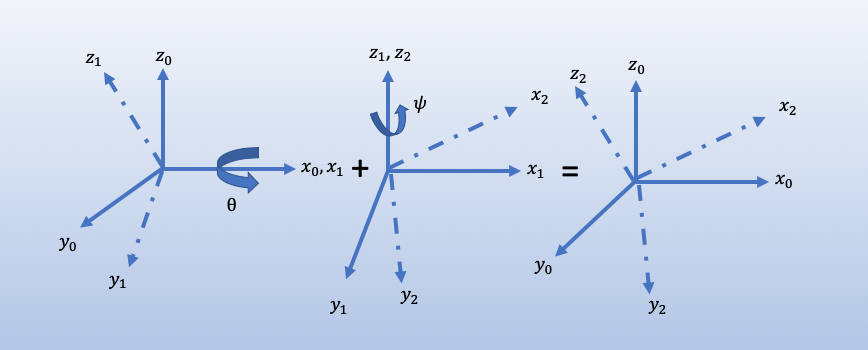
\includegraphics[width=\columnwidth]{figures/compoz.png}
	\caption{Illustration of composition of rotations about a \textbf{current axis}.}
	\label{fig:compoz}
\end{figure}
%
\begin{align}
R &= R_{x, \theta} R_{z, \psi} 
%
&= \left(\begin{array}{ccc}
1 & 0 & 0 \\
0 & c_\theta & -s_\theta \\
0 & s_\theta & c_\theta
\end{array}\right) 
%
\cdot
%
\left(\begin{array}{ccc}
c_\psi & -s_\psi & 0 \\
s_\psi & c_\psi & 0 \\
0 & 0 & 1
\end{array}\right)
%
&= \left(\begin{array}{ccc}
c_\psi & -s_\psi & 0 \\
0 & c_\theta c_\psi &  -s_\theta \\
s_\theta s_\psi & s_\theta c_\psi & c_\theta 
\end{array}\right)
\end{align}
%
Notice how the order of multiplication is carried out, owing to the axis about which we are making the transformation. 

\noindent 
\begin{homework}
	Carry out the transformation above in reverse order. What do you notice?
\end{homework} 


\section{Parameterization of Rotations $\in SO(3)$}
%
\subsection{Axis-Angle Parameterizations}
The exponential coordinates are the \textit{canonical} coordinates of the rotation group. A rigid body has at most three rotational degrees of freedom so that we need at most three variables to denote its orientation in the world. For the matrix 
%
\begin{align}
	R = \begin{bmatrix}
	r_{11} & r_{12} & r_{13} \\
	%
	r_{21} & r_{22} & r_{23} \\
	%
	r_{31} & r_{32} & r_{33} \\
	\end{bmatrix}
\end{align}
%
so that equating the foregoing with the exponential map for a rotation about $\theta$ around an axis $\omega$ as yields
%
\begin{align}
	e^{\hat{\omega}\theta}  &= \identity + \hat{\omega} \sin \theta + \hat{\omega}^2(1 - \cos \theta) \\%
	%
	& = \begin{bmatrix}
	\omega_y^2 v_\theta + c_\theta  & \omega_x\omega_y v_\theta - \omega_z s_\theta & \omega_x \omega_z v_\theta + \omega_y \, s_\theta \\
	 %
	\omega_x \omega_y v_\theta + \omega_z s_\theta  & \omega_y^2 v_\theta+ c_\theta & \omega_y \omega_z v_\theta - \omega_x s_\theta \\
	%
	\omega_x \omega_z v_\theta - \omega_y s_\theta  & \omega_y \omega_z v_\theta + \omega_x s_\theta & \omega_z^2 v_\theta + c_\theta
	\end{bmatrix},
	\label{eq:axis_angle}
\end{align}
%
where we have used $v_\theta = 1 - \cos \theta$. Therefore, we have
%
\begin{align}
	trace(R) = r_{11}  + r_{22}  + r_{33} = 1 + 2 c_\theta
\end{align}
%
Inspecting the matrix of \eqref{eq:axis_angle}, we have the angle of rotation in terms of the three components of the rotation matrix as 
%
\begin{align}
	\theta = \cos^{-1}\left(\dfrac{trace(R) -1}{2}\right)
	\label{eq:angle_part}
\end{align}
% 
where $\theta$ is defined under the constraint, $-2\pi n \le \theta \le 2 \pi n$  owing to the special property of $R$.\footnote{Since $R$ preserves lengths and $\text{ det } R = + 1$, the eigenvalues of R have a unit magnitude and occur in complex conjugate pairs. This implies $-1 \le trace(R) \le 3$}. 

\noindent 
\begin{homework}
	Verify by equating the off-diagonal terms that 
	%
	\begin{align}
	\omega = \frac{1}{2 \sin \theta} \left(
	\begin{array}{c}
	r_{32} - r_{23} \\
	%
	r_{13} - r_{31} \\
	%
	r_{21} - r_{12}
	\end{array} \right)
	\label{eq:axis_part}
	\end{align}
	%
	\noindent suppose $\theta \neq 0$. 
	Equation \eqref{eq:angle_part} together with \eqref{eq:axis_part} are what we call the \textit{axis-angle representation}.
\end{homework} 
%

\subsection{Euler Angles}
%
The \textit{Euler Angles} are particularly useful for specifying the orientation of a a coordinate frame $J$ with respect to $I$. To do this, we start as follows (see \autoref{fig:zyz} for reference):
%
\begin{figure}[tb!]
	\centering
	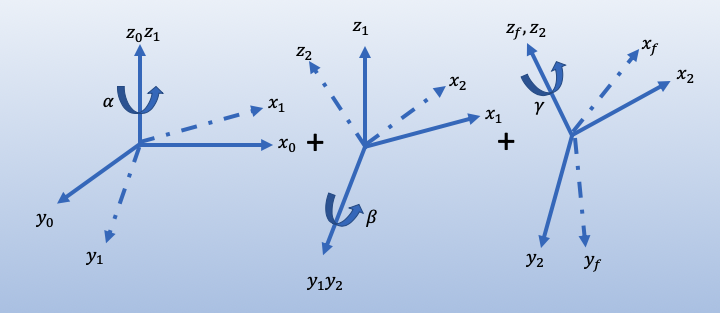
\includegraphics[width=.8\columnwidth]{figures/zyz.png}
	\caption{An illustration of the ZYZ rotation angles}
	\label{fig:zyz}
\end{figure}
\begin{itemize}
	\item we orientate frame $J$ with frame $I$ so that the two frames are coincident by rotating by the $z$ axis about an angle $\alpha$;
	%
	\item we then rotate about the \textit{new} y-axis of $J$ by an angle $\beta$;
	%
	\item lastly, we rotate about the new z-axis of rge frame $J$ by an angle $\gamma$ 
\end{itemize}
%
so that altogether, we have a rotation $R_{ij}(\alpha, \beta, \gamma)$ given as 
%
\begin{align}
	R_{ij}(\alpha, \beta, \gamma) &= R_z(\alpha) R_y(\beta) R_z(\gamma) \\
	%
	& = \begin{bmatrix}
	c_\alpha & -s_\alpha & 0 \\
	%
	s_\alpha & c_\alpha & 0 \\
	%
	0 & 0 & 1
	\end{bmatrix}
	%
	\begin{bmatrix}
	c_\theta  & 0 & s_\theta\\
	%
	0  & 1 & 0 \\
	%
	-s_\theta  & 0 & c_\theta 
	\end{bmatrix} \nonumber \\
	%
	&= \begin{bmatrix}
	c_\alpha c_\beta c_\gamma - s_\alpha s_\gamma & -c_\alpha c_\beta s_\gamma - s_\alpha c_\gamma & c_\alpha s_\beta \\
	%
	s_\alpha c_\beta c_\gamma + c_\alpha s_\gamma & -s_\alpha c_\beta s_\gamma + c_\alpha c_\gamma  & s_\alpha s_\beta \\
	%
	-s_\beta c_\gamma & s_\beta s_\gamma & c_\beta
	\end{bmatrix} 
	\label{eq:zyz}
\end{align}
%
where as before the abbreviations $c_\alpha, s_\alpha$ are abbreviations for $\cos \alpha$ and $\sin \alpha$. Euler angles arise when we need to recover the $\alpha, \beta, \gamma$ angles from \eqref{eq:zyz}. Suppose that $r_{13}$ and $r_{23}$ are both  $\neq 0$, we find that $c_\beta \neq \pm 1$ and thus with the knowledge that $\sin \beta >0$ given \eqref{eq:euler_a}, we find that , 
%
\begin{subequations}
\begin{align}
\beta &= \arctan 2(r_{33}, \sqrt{1 - r_{33}^2})  \label{eq:euler_a}\\
\alpha &= \arctan 2(r_{23}/\sin \beta, r_{13}/\sin \beta) \label{eq:euler_b} \\
\gamma &= \arctan 2 (r_{32}/\sin \beta, -r_{31}/\sin \beta)
\end{align}
\label{eq:euler}
\end{subequations}
%
where $\arctan2(y, x)$ computes $\tan^{-1}(y/x)$, determining the quadrant of the angle based on the sign of $x$ and $y$.
%
When $\sin \beta < 0$, we find that 
%
\begin{subequations}
	\begin{align}
	\beta &=  \arctan2(r_{33}, -\sqrt{1 - r_{33}^2})  \label{eq:euler_neg_a}\\
	\alpha &= \arctan 2(-r_{23}/\sin \beta, -r_{13}/\sin \beta) \label{eq:euler_neg_b} \\
	\gamma &= \arctan 2 (-r_{32}/\sin \beta, r_{31}/\sin \beta)
	\end{align}
	\label{eq:euler_neg}
\end{subequations}
%
implying that \textit{the Euler angles are not unique} owing to the sign of the angle about which the $y$ axis rotates. 

\noindent 
\begin{homework}
	What happens when $r_{13} = r_{23} = 0$? Can you write out the rotation matrix as well as the euler angles for this situation?
\end{homework}

In the scenario that results from homework viii, there will be infinitely many solution owing to the fact that only $\alpha + \beta$ only can be determined. This infinite solutions occur wehn $\rot = \identity$ and an example scenario of when this occurs is when $(\alpha, 0, -\alpha)$.

Using the $ZYZ$ angles are not the only way of parameterizing the rotation matrix. We could permute the order of rotation or rotate successively about different axis. Examples include $ZYX$ axes rotations (or Fick angles) and the $YZX$ axes parameterization or Helmholtz angles. In general robotics speak, note that the \textit{$ZYX$  angles are otherwise referred to as the yaw, pitch and roll angles, wherein the rotation matrix $\rot_{ij}$ is defined by rotating about the $x-$axis in the body frame (roll), then the $y-$axis in the body frame (pitch), and finally the $z-$axis in the body frame (yaw). } An advantage of the Fick angle  and Helmholtz angle parameterization is that they avoid singularity at $\rot = \identity$ though they do contain singularities at other configurations.

\subsection{Quaternions}
%
Rather than use rotation matrices to represent orientations, a more effective approach of representing orientations are \textit{quaternions}. Intead of locally parameterizing the \textit{SO(3)} Lie group, quaternions, unlike rotation matrices, globally parameterize the \textit{SO(3)} Lie Group. Formally, we represent a quaternion as follows:
%
\begin{align}
	Q = q_0 + q_x \bm{i} + q_y \bm{j} + q_z \bm{k} , \quad {q_i}_{\{i = 0, \cdots, 3\}} \in \bb{R}
\end{align}
%
where $q_0$ is the scalar component of $Q$ and $\bm{q} = (q_x, q_y, q_z)$ is the vector component.

The \textit{unit quaternions} are the subset of all $Q \in \bb{Q}$ such that $\|Q\| = 1$; for a rotation matrix $R = \text{exp}(\hat{\omega}\theta)$, we have the unit quaternion as 
%
\begin{align}
	Q = \left(\cos(\theta/2), \omega \sin \left(\theta/2\right) \right),
\end{align}
%
where $\omega \in \bb{R}^3$ is the axis of orientation and $\theta \in \bb{R}$ is the angle of rotation.

\begin{tcolorbox}[title=Summary of Parameterizations]
	Rotation matrices can be parameterized in one of many ways depending on our use case. The common examples of parameterizations are 
	%
	\begin{inparaenum}[\itshape (1)\upshape] \newline
		\item Axis-Angle representation; \newline
		\item Euler  angles ($ZYZ$) representation; \newline
		\item Fick  angles (\ie $ZYX$ or yaw, pitch and roll)  representation; \newline
		\item Helmholtz angles (or $YZX$) angles representation; and \newline
		\item Quaternions.
	\end{inparaenum}
	
\end{tcolorbox}

\section{Homogeneous Coordinates}
%
For a point $q \in \bb{R}^3$, we represent the \textit{homogeneous coordinates} of point $q$ as 
%
\begin{align}
	\bar{q} = \left(\begin{array}{cccc}
	q_x &  q_y & q_z & 1
	\end{array}\right)^T
\end{align}
%
whose origin has the following coordinates
%
\begin{align}
\bar{O} = \left(\begin{array}{cccc}
0 &  0 & 0 & 1
\end{array}\right)^T.
\end{align}
%
For vectors, it would suffice for us to write
%
\begin{align}
	\bar{v} =  \left(\begin{array}{cccc}
	v_x &  v_y & v_z & 0
	\end{array}\right)^T
\end{align}
%
where the last element is zero because a vector is the difference of two points.
%
\begin{tcolorbox}[title=Vectors and Points]
	\begin{itemize}
		\item The sum or difference of two vectors results in a vector
		%
		\item The difference between two points is a vector
		%
		\item The sum of two points do not exist
	\end{itemize}
\end{tcolorbox}
%
We now define the homogeneous transformation of a point $q_j$ in frame $J$ with respect to a coordinate frame $I$ with $p_{ij}$ being the distance between $q_i, \text{ and } q_j$,  and $R_{ij}$ being the rotation matrix that transforms points in frame $J$ to points in frame $I$. We write 
%
\begin{align}
	q_i = p_{ij} + R_{ij} q_j
\end{align}
%
or more appropriately
%
\begin{align}
\left(\begin{array}{c}
q_i \\ 1
\end{array}\right) = \left(\begin{array}{cc}
R_{ij} & p_{ij} \\
%
0 & 1
\end{array}\right) \left(\begin{array}{c}
q_j \\ 1
\end{array}\right) 
\end{align} 
%
which implies that $\bar{q} = \bar{\homo}_{ij} \bar{q}_j$. We say $\bar{g}_{ij}$ is the \textit{homogeneous representation of $\homo_{ij} \in SE(3)$}. 

Similar to rotation matrices, rigid body transformation matrices can be composed to form new rigid body transformations. So, suppose we have the $g_{jk}$ which is the transformation of a body $K$ relative to body $J$ and $g_{ij}$ which is the transformation of body $J$ relative to body $I$, then we can find the configuration of $K$ relative to $I$ as follows
%
\begin{align}
	\bar{g}_{ik} = \bar{g}_{ij} \bar{g}_{jk} 
	&= \left(\begin{array}{cc}
	R_{ij} & p_{ij} \\
	%
	0 & 1
	\end{array}\right)
	%
	\left(\begin{array}{cc}
	R_{jk} & p_{jk} \\
	%
	0 & 1
	\end{array}\right) \\
	%
	&= \left(\begin{array}{cc}
	R_{ij} R_{jk} & R_{ij} p_{jk} + p_{ij}\\
	%
	0 & 1
	\end{array}\right).
	\label{eq:transform_compoz}
\end{align}
%
Since \eqref{eq:transform_compoz} is a form of \eqref{eq:special_euclid3}, we conclude that the composition of rigid body transformations and $I_{4\times 4}$ is in the special Euclidean group as well. In addition, 
%
\begin{align}
	\homo^{-1} = \left(R^Tp, R^T\right).
	\label{eq:compact_transform}
\end{align}

\section{Rigid Body Velocities}
%
We are concerned with the velocity of a rigid body with motion described by a time-parameterized curve $\homo(t) \in SE(3)$. For a start, we will consider the trajectory motion of an object frame $J$ whose origin is at a frame $I$ and it is rotating relative to the fixed frame $I$. We call frame $I$ the \textit{spatial frame} and the frame $J$, the \textit{body frame}. 

\subsection{Rotational Velocities}
%
For a point $q$ whose coordinates $q_j$ are fixed in the body frame, a path in spatial coordinates is followed given by 
%
\begin{align}
	q_i(t) = R_{ij}(t) q_j.
	\label{eq:body_spatial}
\end{align}
%
The velocity in spatial coordinates is 
%
\begin{align}
	v_{q_i}(t) = \frac{\partial}{\partial t} q_i(t) = \dot{R}_{ij}(t) q_j.
\end{align}
%
We see that $\dot{R}_{ij}$ maps the body coordinates, $q_j$ to the spatial velocity of $q$. We would like to develop a more compact representation of the orientation of the point $q$ relative to the spatial frame $I$ by exploiting the special structure of $\dot{R}_{ij}$.  Thus, we write 
%
\begin{align}
	v_{q_i}(t) = \dot{R}_{ij}(t) R_{ij}^{-1}(t) R_{ij}(t) q_j.
	\label{eq:angular_vel}
\end{align}
%
We define the \textit{instantaneous spatial angular velocity} $\hat{\omega}^s_{ij} \in \bb{R}^3$ as seen in the spatial frame $I$ as 
%
\begin{align}
	\hat{\omega}^s_{ij}(t) =	\dot{R}_{ij}(t) R_{ij}^{-1}(t) %\in so(3)
\end{align}
%
and we define the \textit{instantaneous body angular velocity}  as seen in the body frame $J$ as
%
\begin{align}
\hat{\omega}^b_{ij}(t) = R_{ij}^{-1}(t) \dot{R}_{ij}(t) %\in so(3) %\hat{\omega}^s_{ij} R_{ij}(t)
\end{align}
%
We define the body angular velocity  as viewed from the instantaneous body frame $J$ as 
%
\begin{align}
\hat{\omega}^b_{q_b} = R^{-1}_{ij} \hat{\omega}^s_{ij} R_{ij}, \text{ or }  \hat{\omega}^b_{ij} = R^{-1}_{ij} \hat{\omega}^s_{ij},
\end{align}
%
so that the body angular velocity can be recovered from the spatial angular velocity by rotating the angular velocity vector into the instantaneous body frame. Thus, \eqref{eq:angular_vel} becomes 
%
\begin{align}
v_{q_i}(t) = \hat{\omega}^s_{ij}(t) R_{ij}(t) q_j = \hat{\omega}^s_{ij}(t) \times q_i(t)
\label{eq:angular_vel_compact}
\end{align}
%
Similarly, the velocity in the frame $J$ can be derived from \eqref{eq:body_spatial} as
%
\begin{subequations}
	\begin{align}
	q_j &= R_{ij}^{-1}(t) q_i(t) \\
	v_{q_j}(t) &= \dot{R}_{ij}^T(t) \, v_{q_i}(t) = \omega_{ij}^b(t) \times q_j.
	\end{align}
\end{subequations}
%
Thus we have the compact description of the rigid body particles' velocities in both the body and spatial angular frames as $\omega_{ij}^b$ and $\omega_{ij}^s$.

\noindent 
\begin{homework}
	Consider the motion of a point body about the $x$ axis of an orthogonal triad with respect to a certain spatial frame located at $O(0,0,0)$. Determine the body and spatial velocities of the point with respect to the origin, $O$.
\end{homework}

\subsection{Rigid Body Velocity}
%
We shall denote the rigid body motion of a frame $J$ attached to a body so that is it fixed relative to a frame $I$ by ${\homo}_{ij}(t)$. We write the velocity in the spatial frame as $	\dot{\homo}_{ij} \homo_{ij}^{-1} $ which is symbolically $\left(\dot{p}_{ij}, \dot{R}_{ij}\right) \cdot \left({R}_{ij}^T, -{R}_{ij}^Tp_{ij}\right)$ following the notation we introduced in \eqref{eq:compact_transform}. This has an isomorphism of a twist and it is given by 
%
\begin{tcolorbox}[title=Twist in Spatial Frame]
	\begin{align}
	\eta_{ij}^s = \dot{\homo}_{ij} \homo_{ij}^{-1} 
	&= \begin{bmatrix}
	{\omega}_{ij}^s & {v}_{ij}^s \\
	%
	0 & 0
	\end{bmatrix} = 
	\begin{bmatrix}
	\dot{\rot}_{ij} \rot_{ij}^T  & -\dot{\rot}_{ij} \rot_{ij}^T  p_{ij} + \dot{p}_{ij}\\
	%
	0 & 0
	\end{bmatrix} \in \mathfrak{se(3)} 
	\label{eq:twist_spatial}
	\end{align}
\end{tcolorbox}
%
whereupon the twist coordinates $\xi^s \in \bb{R}^6$ in the body frame can be recovered as 
%
\begin{align}
	\left(
	\begin{array}{c}
	{v}_{ij}^s  \\ {\omega}_{ij}^s 
	\end{array}
	\right) = \left(
	\begin{array}{c}
	-\dot{\rot}_{ij} \rot_{ij}^T  p_{ij} + \dot{p}_{ij} \\ 	(\dot{\rot}_{ij} \rot_{ij}^T)^{\vee}
	\end{array}
	\right) 
\end{align}
%
Similarly, in body coordinates, we find that the twist is given by 
%
\begin{tcolorbox}[title=Twist in Body Frame]
	\begin{align}
	\eta_{ij}^b = \homo_{ij}^{-1} \dot{\homo}_{ij} 
	&= \begin{bmatrix}
	{\omega}_{ij}^b & {v}_{ij}^b \\
	%
	0 & 0
	\end{bmatrix} = 
	\begin{bmatrix}
	\dot{\rot}_{ij} \rot_{ij}^T  & \rot_{ij}^T  p_{ij} \dot{p}_{ij}\\
	%
	0 & 0
	\end{bmatrix} \in \mathfrak{se(3)} 
	\label{eq:twist_body}
	\end{align}
\end{tcolorbox}
%
whereupon the twist coordinates $\xi^b \in \bb{R}^6$ in the body frame can be recovered as 
%
\begin{align}
\left(
\begin{array}{c}
{v}_{ij}^b  \\ {\omega}_{ij}^b 
\end{array}
\right) = \left(
\begin{array}{c}
-\dot{\rot}_{ij}^T \dot{p}_{ij} \\ 	(\rot_{ij}^T \, \dot{\rot}_{ij})^{\vee}
\end{array}
\right) 
\end{align}
%
Furthermore, we have that 
%
\begin{align}
	\eta_{ij}^s = 
	\left(
	\begin{array}{cc}
	-\dot{\rot}_{ij} & \hat{p}_{ij} {\rot}_{ij} \\ 	0 & \rot_{ij}
	\end{array}
	\right) 
	%
	\left(
	\begin{array}{c}
	{v}_{ij}^b  \\ {\omega}_{ij}^b 
	\end{array}
	\right).
	\label{eq:twist_equiv}
\end{align}
%

\noindent 
\begin{homework}
	Confirm equations \eqref{eq:twist_spatial}, \eqref{eq:twist_body} and \eqref{eq:twist_equiv}.
\end{homework}


The matrix which transforms from the body coordinate frame to the spatial velocity frame is the so-called \textit{adjoint transformation} of $\homo$ (\cf \autoref{fig:lienotations}), defined as 
%
\begin{align}
	Ad_\homo  = \left(\begin{array}{cc}
	R & \hat{p} R \\
	%
	0 & R
	\end{array}\right)
\end{align}
%
and whose inverse is given by 
%
\begin{align}
	Ad_\homo^{-1}  = \left(\begin{array}{cc}
R^T & -(R^Tp)^\wedge R^T \\
%
0 & R^T
\end{array}\right) 
%
= \left(\begin{array}{cc}
R^T & -R^T \hat{p} \\
%
0 & R^T
\end{array}\right) = Ad_{\homo^{-1}}
\end{align}

%\subsection{Lab Exercise in ROS}
%
%Here, we will use the \textsc{geometry\_msgs} package which. The idea is to introduce you to the way the theory we have been working upon all along translate into practice. It is assumed that you already have any pf \textsc{ros kinetic or up to ros bouncy} installed on a ubuntu computer. 
%\todo{To be further developed.}